\chapter{Tercera Iteración: El Emulador y los editores}

Como se explica en el apartado \ref{metodologiadedesarrollo}, en donde se expone la metodología de desarrollo utilizada para el proyecto, este pasa a lo largo de tres grandes iteraciones para completarse. En este apartado se explican los detalles implementados en la tercera iteración, es decir, la generación de un emulador de juegos e eAdventure, utilizando el núcleo de ejecución \textit{Runner} explicado en el apartado \ref{runnerit2}, y el modelo de datos de eAdventure explicado en \ref{coreit2}; además de la generación de editores para el editor de uAdventure desarrollado por Piotr Marszal. 

\section{El Emulador de Juegos}
\label{emulatorit3}

Uno de los principales problemas de todo software consiste en que el presupuesto que se invierte en el desarrollo de dicho software no debe invertirse por completo en su desarrollo, pues la vida útil del mismo durará varios años más, en los que debe haber un mantenimiento y soporte para dicho software. El software producido por eAdventure, en muchos casos, hace años que dejó de tener soporte, pues no sólo los desarrolladores abandonaron los proyectos, sino que eAdventure no sufre ninguna actualización desde el 29 de Octubre de 2012, y todos los errores que han surgido, y los problemas de soporte que tiene en diferentes dispositivos han limitado la vida útil del software producido con eAdventure, y su ciclo de vida.

uAdventure, construido sobre Unity3D permite abrir proyectos de eAdventure, y videojuegos ya generados, dando la posibilidad de modificarlos y probarlos sobre el nuevo núcleo de ejecución, ampliando y simplificando el ciclo de vida del videojuego. Tras haber abierto dicho juego, mediante las herramientas de compilación de Unity se puede generar un paquete ejecutable con el juego en su interior.

No obstante, muchos proyectos han sido completamente abandonados, y es posible que nadie decida transformar un juego o que, por desconocimiento de su existencia, no se transforme a uAdventure. Por todo ello, este \textit{framework} puede ser compilado en sí mismo como un emulador de juegos de eAdventure, permitiendo al usuario explorar su sistema de ficheros, e importar de forma sencilla aquellos juegos que desee jugar.

Este emulador evoluciona de una prueba incluida en la clase controladora del juego en el prototipo generado en la primera iteración. Esto consistía en permitir al usuario seleccionar un juego de una lista de juegos disponibles en lugar de lanzar directamente un juego especificado en la clase controladora. En este primer prototipo la interfaz era muy sencilla, sin opciones, y no permitía técnicamente importar juegos, sino que debían de importarse descomprimiendo los juegos en una carpeta determinada del sistema de ficheros. Además, incluía un diálogo de carga que mostraba el progreso de la carga del juego.

Esta primera versión del emulador se muestra en la Figura \ref{betaemuit3}.

\begin{figure}[htb]
	\centerline{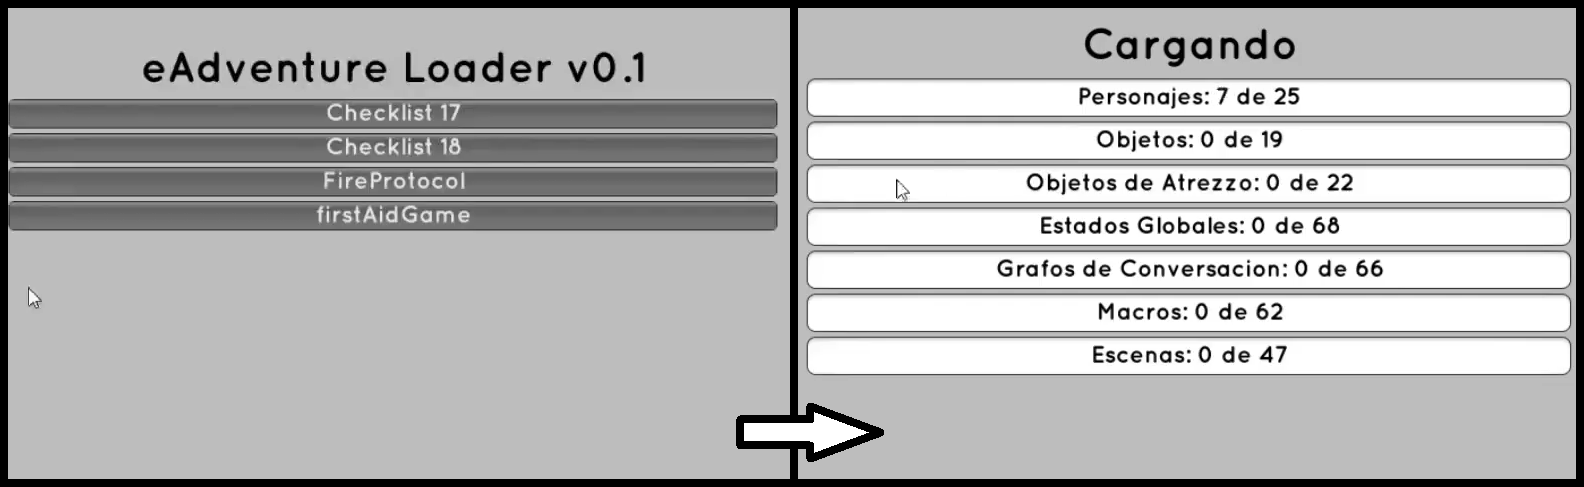
\includegraphics[height=2in]{figures/it3/betaemu.png}}
	\caption[Primer prototipo - Emulador]{La parte de la izquierda muestra el menú principal del primer prototipo del emulador. Una vez seleccionado un juego, se mostraba un diálogo de carga como el que se ve en la parte derecha.}
	\label{betaemuit3}
\end{figure}

No obstante, y dado que esta primera versión del emulador era insuficiente, además de que el diálogo de carga de ficheros no permitía ser ejecutado si se utiliza el sistema de carga de recursos de Unity, \textit{Resources.Load()}, este emulador evolucionó en cinco vistas:

\begin{itemize}
	\item \textbf{Menú Principal}: El menú es la puerta de entrada al emulador. Cuando se pone en funcionamiento muestra en el centro un catálogo de juegos instalados, si los hay. Pulsando sobre cualquiera de estos juegos comienza la ejecución del mismo. Finalmente, en la parte inferior de la vista hay tres botones que permiten acceder a más vistas del emulador. Cada juego presentado en el menú principal tiene un icono que lo representa. La obtención de dicho icono se hace explorando los archivos incluidos dentro del directorio ``/gui/'' en busca de un fichero llamado ``standalone\_game\_icon.png''. Si dicho fichero no existe, se selecciona el icono de la versión de eAdventure con la que fue generado dicho juego, incluido también en el mismo directorio.

\begin{figure}[h!]
	\centerline{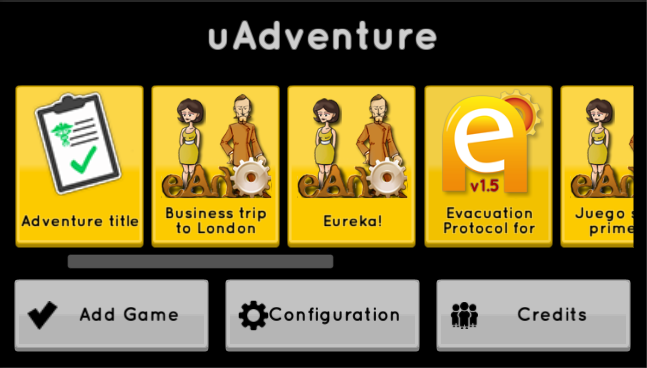
\includegraphics[height=2.5in]{figures/it3/emu-main.png}}
	\caption[Menu Principal - Emulador]{Vista del menú principal del emulador de uAdvneture.}
	\label{emumainit3}
\end{figure}


	\item \textbf{Explorador de Archivos}: Dado que Unity no provee, en tiempo de ejecución, de una manera de seleccionar un fichero del sistema de archivos, se ha implementado desde cero un explorador de archivos. Este permite navegar por carpetas, las cuales se ven en un color amarillo, y seleccionar juegos para ser añadidos. Estos juegos se representan con el icono de un mando de videojuegos, y con un color azul. Tras seleccionar un juego se puede pulsar el botón \textit{Add Game}, que lanza la vista que se presenta a continuación.

\begin{figure}[h!]
	\centerline{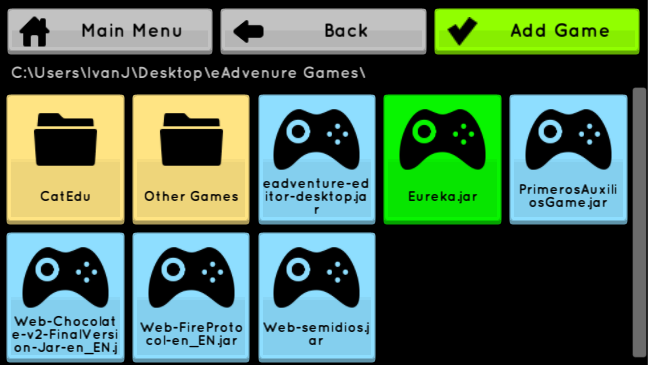
\includegraphics[height=2.3in]{figures/it3/emu-file.png}}
	\caption[Explorador de Archivos - Emulador]{Vista del explorador de archivos del emulador de uAdventure.}
	\label{emufileit3}
\end{figure}

	\item \textit{Importador de juegos}: Pese a que esta sea una de las vistas más sencillas, pues únicamente muestra un texto y una pequeña animación de tres puntos moviéndose, tras esta animación se encuentra el proceso de importado del juego. En el que se descomprimen las partes necesarias, y se borran algunos elementos tras su descompresión. Como se explicó en el apartado \ref{resourcemanagerit2}, la transformación de los vídeos se realizaría en esta escena.
	
\begin{figure}[h!]
	\centerline{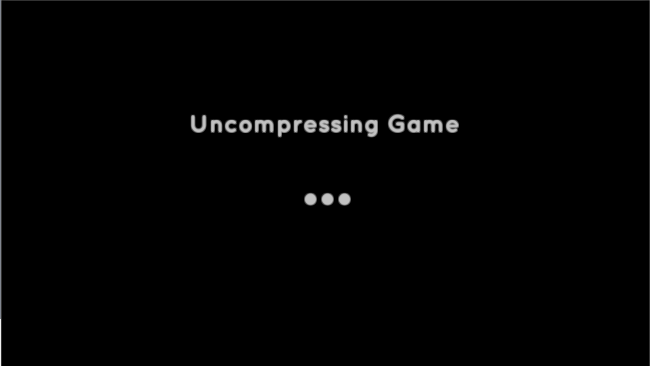
\includegraphics[height=2.3in]{figures/it3/emu-loader.png}}
	\caption[Importador de Juegos - Emulador]{Vista del importador de juegos del emulador de uAdventure.}
	\label{emuloaderit3}
\end{figure}
	
	\item \textit{Configuración}: La ventana de configuración provee al usuario de la capacidad de poder modificar el funcionamiento del intérprete, pudiendo configurar tres apartados: Gráficos, Sonido y Otros. Dentro del apartado gráfico se permite la posibilidad de deshabilitar los \textit{Shaders} explicados en el apartado \ref{apearanceseccionit2}, así como deshabilitar los vídeos, o las animaciones. Dentro del apartado de sonido se permite configurar el uso de audio, así como su volumen y si se desea, forzar el uso de \textit{Text To Speech}, texto hablado. Finalmente, en el apartado de otras configuraciones, se permite modificar la velocidad del texto en las burbujas, así como la posibilidad de dehabilitar RAGE, o la persistencia de ficheros multimedia, para reducir el uso de memoria de la aplicación.
	
\begin{figure}[h!]
	\centerline{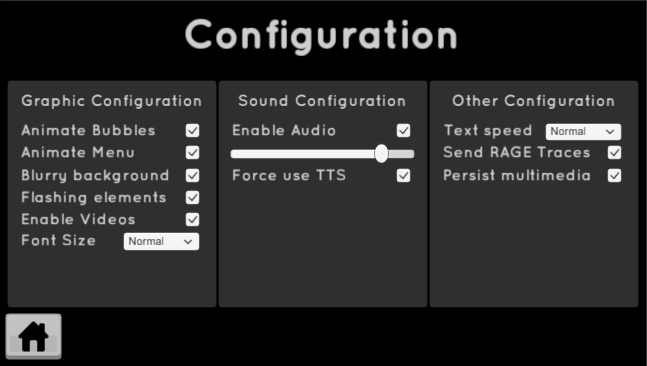
\includegraphics[height=2.3in]{figures/it3/emu-config.png}}
	\caption[Configuración - Emulador]{Vista de configuración del emulador de uAdventure.}
	\label{emuconfigit3}
\end{figure}
	
	\item \textit{Créditos}: La vista de créditos contiene el listado de las personas que han participado, dirigido o realizado aportaciones tanto a uAdventure como a eAdventure.
	
\begin{figure}[h!]
	\centerline{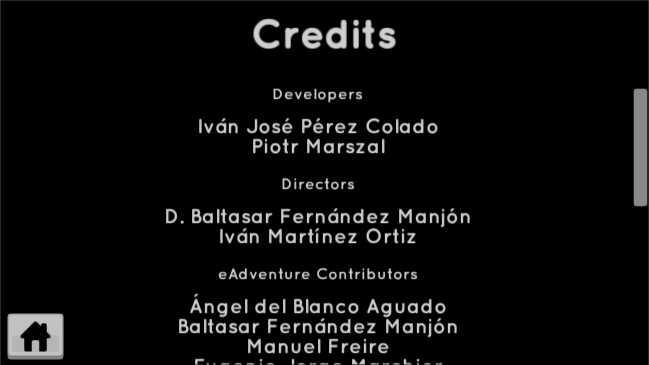
\includegraphics[height=2.3in]{figures/it3/emu-credits.png}}
	\caption[Créditos - Emulador]{Vista de los créditos presentados en el emulador de uAdventure.}
	\label{emucreditsit3}
\end{figure}

\end{itemize}

\section{Los Editores de Secuencias}
\label{sequencesit3}

Como parte del proceso de integración de los proyectos, y para realizar un aporte comparable al esfuerzo que Piotr Marszal había realizado al importar el modelo de datos de eAdventure, en el desarrollo de este proyecto se generaron dos editores basados en ventanas para la edición de las secuencias.

Dada la experiencia de generación de editores de este estilo obtenida durante el desarrollo del TFG IsoUnity, que consistía en la generar un editor de videoaventuras en tercera persona con estilo isométrico, en el que se incluyen editores que presentan similitudes con dichas necesidades, el desarrollo de dichos editores será más sencillo.

Las clases de eAdventure que requieren editores son: los efectos, que pese a ser lineales, se plantea la posibilidad de incluir bifurcaciones que los transformen en un grafo en un futuro; Las conversaciones, que son grafos de diálogo con nodos de conversación que incluyen diálogo o opciones de respuesta; y el editor de condiciones, que al ser tan pequeño se explicará como parte del editor de efectos.

Para el desarrollo de cada uno de estos editores se implementarán tres clases cruciales:

\begin{itemize}
	\item La ventana principal del editor, que es capaz de gestionar la secuencia en si misma, compuesta por un listado de nodos, y de mantener en orden las ventanas que representan los editores individuales de cada uno de los nodos.
	
	\item Una interfaz que permita implementar editores para los nodos, con métodos para pintarse utilizando la \textit{GUI} de editor de Unity, y métodos que permiten identificar si un editor sirve para representar un tipo de nodo, y clonarse a si mismo.
	
	\item Finalmente, una factoría que explore el espacio de nombres utilizando \textit{Linq}, en busca de editores que implementen la interfaz para generar editores de nodo. Dicha factoría también tiene que proveer un listado de los editores disponibles, así de facilidades para instanciar un editor para un nodo concreto. Existen detalles acerca de la implementación de factorías utilizando esta técnica en el apartado \ref{linqit1}
\end{itemize}

Con estas tres clases, ya se pueden generar editores individuales para los nodos, consiguiendo un editor de secuencias muy extensible, preparado para añadir nuevos editores de forma sencilla y sin necesidad de modificar ninguna de las clases. Generando una nueva clase que implemente la interfaz del editor, este ya la identificaría y añadiría a su listado de editores disponibles.

\subsection{El Editor de Efectos}

Entre los editores de secuencias implementados, el más sencillo, pero a su vez más largo de implementar es el editor de efectos, pues estos son una secuencia lineal, no son ni árboles, ni grafos, por lo que la implementación de un editor con ventanas lineal se plantea sencilla. Sin embargo, la cantidad de editores de efectos que se deben implementar es muy elevada, pues existen multitud de efectos que implementan la interfaz \textit{AbstractEffect}.

Para la implementación de esta ventana de editor, se extiende la clase abstracta \textit{EditorWindow} que provee una serie de métodos que, de implementarse, permiten la generación de una nueva ventana para el editor. En primer lugar, una función \textit{Init()} que inicializa la ventana para un efecto dado. Una funcion \textit{nodeWindow(int id)} que se encarga de gestionar cada ventana individualmente. Unas funciones \textit{CreateWindows()} y \textit{CreateWindow(AbstracEffect effect)}, que son las encargadas de generar las ventanas para los efectos. Una funcion \textit{curveFromTo()} que genera una línea entre dos ventanas, y finalmente, la función \textit{OnGUI()} que ejecuta todo lo anterior para generar la ventana.

En la Figura \ref{mainwindow-effecteditor-it3} se ve una secuencia de efectos sencilla, compuesta por 5 efectos en los que se establece valor para unas variables, el jugador habla, y finalmente, se lanza una conversación completa. El menú desplegable muestra todos los editores de efectos implementados. En la parte de arriba de la Figura se observa un botón muy ancho con el texto ``New Effect'', que sirve para añadir un nuevo nodo a la lista de efectos. En esta ventana, las subventanas que permiten la edición de efectos se pueden mover, por lo que permiten la organización de los mismos de la forma más conveniente.

\begin{figure}[h!]
	\centerline{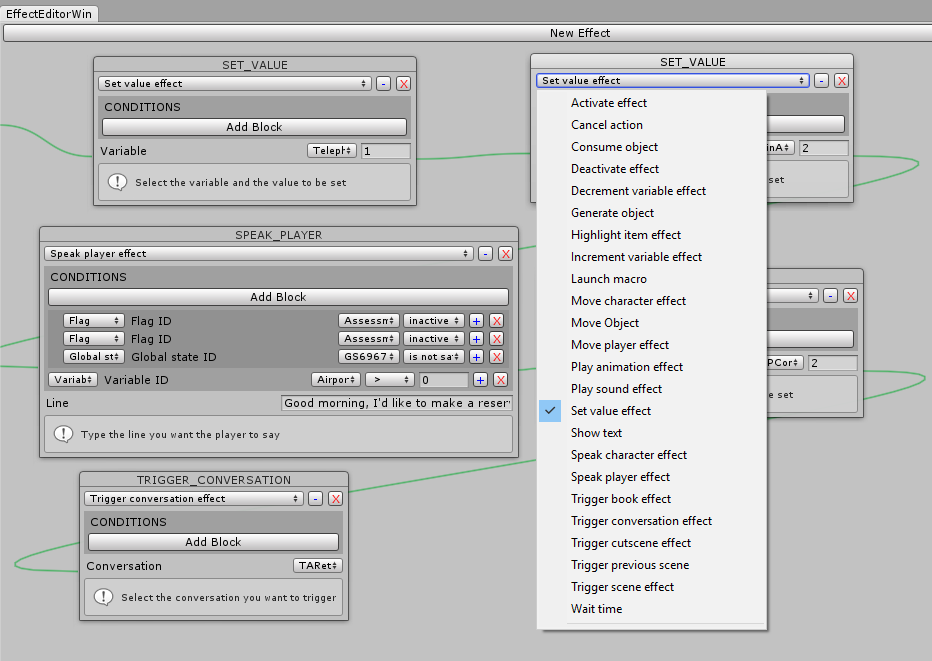
\includegraphics[height=4in]{figures/it3/effecteditorwindow.png}}
	\caption[Ventana Principal - Editor de Efectos]{Ventana principal del editor de efectos.}
	\label{mainwindow-effecteditor-it3}
\end{figure}

En la figura \ref{effect-nodes-it3} se muestra un nodo de efecto que muestra una gran cantidad de condiciones para su ejecución. Este nodo puede reducirse en tamaño para facilitar la edición mediante el botón con el guión de color azul, transformándose en la ventana derecha.

\begin{figure}[h!]
	\centerline{
		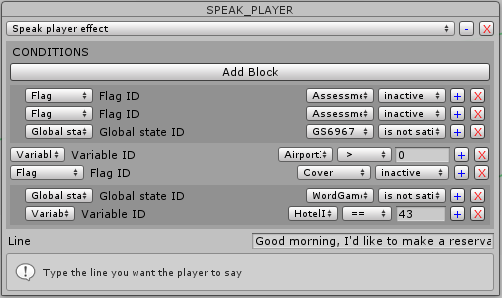
\includegraphics[height=2.5in]{figures/it3/editor-conditions.png}
		
\includegraphics{figures/it3/collapsed-effect.png}
		}
	\caption[Editor de Nodo con condiciones - Editor de Efectos]{Editor de nodo de efecto con condiciones, vista normal y reducida.}
	\label{effect-nodes-it3}
\end{figure}

\subsection{El Editor de Conversaciones}

Pese a que en primera instancia parece que el editor de conversaciones es muy similar al editor de efectos, y aunque visualmente lo sean, las conversaciones son grafos, y la modificación de un editor que trabaja con listas a un editor capaz de trabajar con grafos direccionales no es una tarea trivial. 

Las modificaciones con respecto al editor de efectos están relacionadas con la gestión de ciclos en los grafos, y la posibilidad de generar hijos para nodos concretos, así como permitir al usuario establecer el hijo de un nodo directamente, mostrando en la interfaz cual es la rama de nodos que, si no tiene ningún otro nodo padre, se va a perder, y cual es la nueva rama que se va a establecer como hija de dicho nodo.

Como en el desarrollo de este editor no era tan necesario generar un gran número de editores, pues las conversaciones únicamente están compuestas por editores de diálogos y de opciones, dichos editores cuentan con un acabado mucho más conseguido, reutilizando muchas de las imágenes de la interfaz de eAdventure. Esto se muestra en la Figura \ref{small-dialog-it3}, en la que, además, se muestra lo descrito en el párrafo anterior. La línea azul será el nuevo hijo, y la roja el hijo descartado.

\begin{figure}[h!]
	\centerline{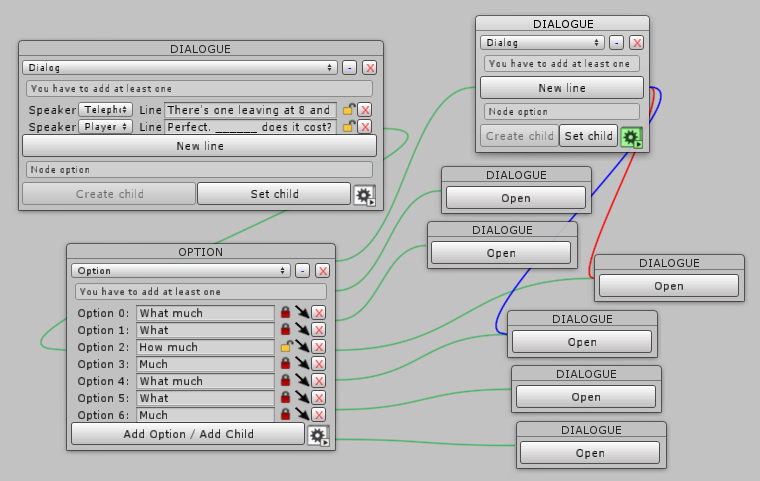
\includegraphics[height=3in]{figures/it3/small-dialog.png}}
	\caption[Pequeño diálogo - Editor de Diálogos]{Pequeño diálogo mostrado en el editor de diálogos.}
	\label{small-dialog-it3}
\end{figure}

Como detalle adicional, se ha generado una clase llamada \textit{NodePosicioner} que, estableciendo un número de nodos, y una altura de la ventana, posiciona automáticamente los nodos en su lugar correspondiente automáticamente, de manera que ver las secuencias es más cómodo si se abren y no existen datos acerca de su posición. Esto se muestra en la figura \ref{circle-nodes-it3}.

\begin{figure}[h!]
	\centerline{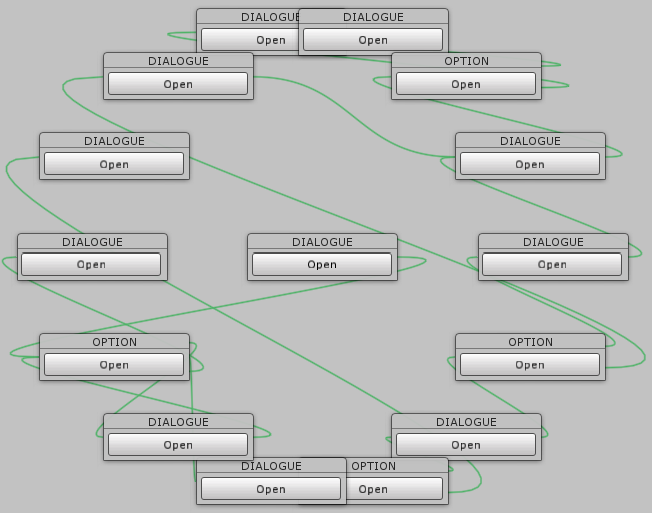
\includegraphics[height=2in]{figures/it3/nodes-circle.png}}
	\caption[Anillo de nodos - Editor de Diálogos]{Posicionamiento automático de nodos en el editor de diálogos.}
	\label{circle-nodes-it3}
\end{figure}

Finalmente, y para mostrar las posibilidades del editor, tenemos la Figura \ref{big-dialog-it3}, en la que se muestra una secuencia muy grande. El icono del candando nos permite la edición de condiciones para mostrar dicha línea, ya sea de opción o de diálogo. La flecha negra permite establecer el nodo hijo para dicha opción directamente. Y por último, el botón de la esquina inferior derecha de cada diálogo permite acceso a los efectos que se ejecutan en dicho nodo. Estas características también se pueden observar en la Figura \ref{small-dialog-it3}

\begin{figure}[h!]
	\centerline{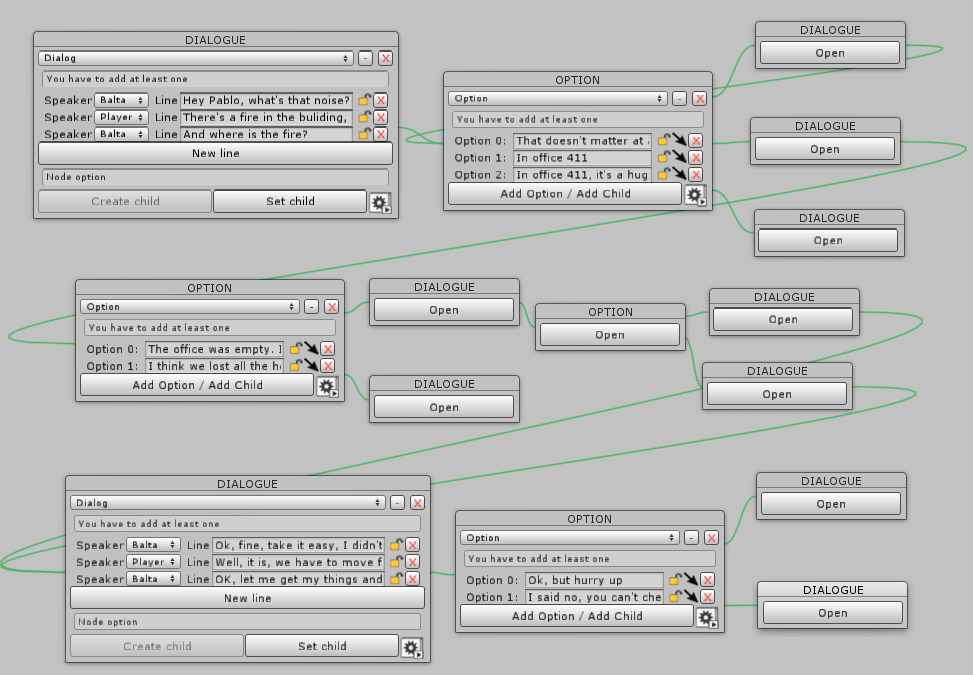
\includegraphics[height=5in]{figures/it3/big-dialog.png}}
	\caption[Gran diálogo - Editor de Diálogos]{Gran diálogo mostrado en el editor de diálogos.}
	\label{big-dialog-it3}
\end{figure}

\newpage

\newpage

\section{El Editor de RAGE}
\label{rageeditorit3}

Como se ha mencionado varias veces a lo largo del documento, especialmente en el apartado \ref{ragetrackerit2}, donde se explica la necesidad de sustituir las funcionalidades de evaluación de alumnos por un sistema más elaborado que el que encontramos en eAdventure; el sistema de evaluación que se utiliza en uAdventure está fuera del mismo, en la nube, y se llama RAGE.

Esta herramienta provee, mediante una interfaz web, una serie de páginas con información importante y gráficas acerca del progreso y evaluación de los alumnos de forma en grupo e individual, permitiendo al profesor enfocar los esfuerzos en aquellos alumnos que hayan quedado rezagados o que demuestren problemas en su aprendizaje.

Pese a que esta interfaz no provee de funcionalidad específica más allá de la que provee la propia interfaz web de RAGE, las clases y funciones implementadas serán utilizadas como trabajo futuro para guardar las configuraciones de evaluación y progreso de videojuegos en RAGE. El propósito de esta ventana se conservará, permitiendo, si se desea, modificar los algoritmos generados por uAdventure para el cálculo de estos elementos.

La Figura \ref{ragewindowit3} muestra las clases que participan en el editor de RAGE. En estas clases se encuentra \textit{RageWindow}, que provee de interfaz y de controlador para la interacción con RAGE, la clase \textit{GameConfiguration}, que es una clase contenedora de los datos de la configuración de un juego en RAGE, con la capacidad de transformarse en JSON, igual que \textit{Warning}. Por otra parte, se encuentra ThreadedNet, una clase que permite realizar peticiones POST y GET de forma paralela utilizando hilos de procesamiento.

\begin{figure}[h!]
	\centerline{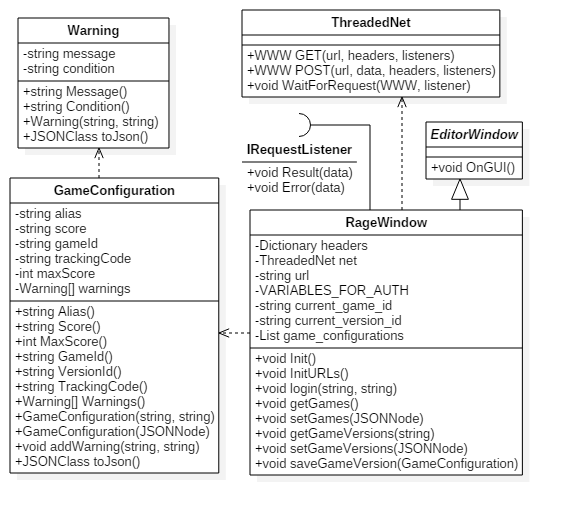
\includegraphics[height=3.5in]{figures/it3/RageWindow.png}}
	\caption[Diagrama de Clases - Editor de RAGE]{Diagrama de clases de las clases que participan en el editor de RAGE.}
	\label{ragewindowit3}
\end{figure}

\chapter{El editor de uAdventure}
\label{piotr}

A lo largo de este documento se referencia en múltiples ocasioes el proyecto de Piotr Marszal. Este proyecto consiste en la reconstrucción del editor de eAdventure dentro de Unity, utilizando las extensiones de editor que Unity permite.

Como uno de los objetivos de este proyecto es dar soporte al ciclo de vida de los juegos de eAdventure, para conseguir que los desarrolladores que crearon juegos en eAdventure no se sientan demasiado fuera de lugar al trabajar con uAdventure, este proyecto ha mantenido una similitud exacta a la hora de recontruir los diferentes menús de la interfaz de eAdventure.

Este tipo de herramientas que extienden la interfaz de Unity son complejas de desarrollar, pues necesitan que el desarrollador trabaje con un enfoque diferente, pues los elementos y clases que participan en el proceso de edición son diferentes de los que participan en la ejecución del juego. Este cambio de mentalidad, junto con los problemas de serialización de elementos hacen que este tipo de proyectos sean complejos de implementar.

Este proyecto ha dado soporte a todas las características de eAdventure, con el aporte adicional de nuevos editores explicados en el apartado \ref{sequencesit3}, en los que la interfaz se ha innovado para mejorar la capacidad de organizar los diferentes nodos que componen las secuencias de elementos.

\begin{figure}[h!]
	\centerline{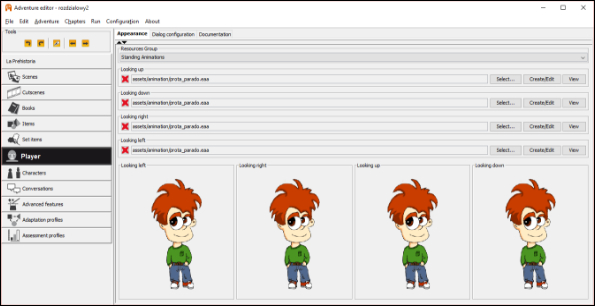
\includegraphics[height=2.5in]{figures/eadventure.png}}
	\caption[uAdventure editor - eAdventure]{Captura del editor original de eAdventure.}
	\label{eadventureeditor}
\end{figure}

Las Figuras \ref{eadventureeditor} y \ref{uadventureeditor} presentan una vista de la misma interfaz, siendo la primera la de eAdventure original y la segunda la del editor reconstruido en Unity.

\begin{figure}[h!]
	\centerline{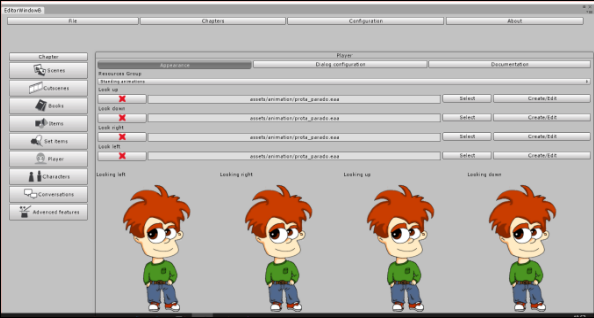
\includegraphics[height=2.5in]{figures/uadventure.png}}
	\caption[uAdventure editor - uAdventure]{Captura del editor reconstruido sobre Unity, uAdventure.}
	\label{uadventureeditor}
\end{figure}

Dentro de la lista de trabajo futuro planteado, se expone la posibilidad de mejorar la interfaz para crear un editor híbrido que una las interfaces de Unity y uAdventure, preparando un perfil de visualización del editor que abstraiga menús y herramientas que puedan distraer a un desarrollador poco experimentando, y dando facilidades para encontrar lo que busque.